\documentclass{ximera}

\newcommand{\RR}{\mathbb R}
\renewcommand{\d}{\,d}
\newcommand{\dd}[2][]{\frac{d #1}{d #2}}
\renewcommand{\l}{\ell}
\newcommand{\ddx}{\frac{d}{dx}}
\newcommand{\dfn}{\textbf}
\newcommand{\eval}[1]{\bigg[ #1 \bigg]}


\author{Jim Talamo}
\license{Creative Commons 3.0 By-NC}


\outcome{Set up an integral to compute a volume of a solid with known cross-sections}

\begin{document}

\begin{exercise}
Throughout this exercise set, we will adopt the following conventions.

\begin{itemize}
\item It is always possible to define remainders for $\sum_{k=n_0}^{\infty} a_k$ \wordChoice{\choice[correct]{$\sum_{k=n_0}^{\infty} a_k$ converges}\choice{we have a formula for the terms in the sequence of partial sums}\choice{whether $\sum_{k=n_0}^{\infty} a_k$ converges or diverges}} . 
\item For a convergent series $\sum_{k=n_0}^{\infty} a_k$, we have the following.

\begin{itemize}
\item The terms in the sequence of \emph{partial sums} $\{s_n\}_{n=n_0}$ are defined from $s_n = \sum_{k=n_0}^n a_k.$
\item  The terms in the sequence of \emph{remainders} $\{r_n\}_{n=n_0}$ are defined from $r_n = \sum_{k=n+1}^\infty a_k.$
\end{itemize}

Note that if the series $\sum_{k=n_0}^{\infty} a_k$ diverges, then the tail $\sum_{k=n+1}^{\infty} a_k$ also diverges, so we cannot assign a value to $r_n$ in this case!

\item This convention lets us split up the series $\sum_{k=1}^{\infty} a_k$ into an ``approximation plus an error'' in the following sense.

\begin{image}
  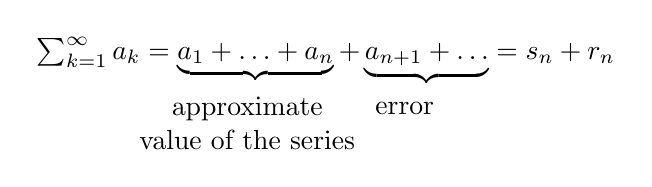
\begin{tikzpicture}
        \node at (0,0) {
          $ \sum_{k=1}^{\infty} a_k=\underbrace{a_1+\ldots +a_n}+ \underbrace{a_{n+1}+ \ldots} = s_n+r_n$};
        \node at (1,-.6) { error};
       
        \node at (-1,-.6) {approximate };
        \node at (-1,-1) {value of the series };
                
      \end{tikzpicture}
  \end{image}
  
Notice that the lower index in the sum for $r_n$ always starts at $n+1$ so we can write the series $ \sum_{k=1}^{\infty} a_k$ as $s_n +r_n$.
  
  We do this because we want to approximate the \emph{infinite} series $\sum_{k=1}^{\infty} a_k$ by the \emph{finite} one $ \sum_{k=1}^{n} a_k$.  The remainder term $r_n$ will tell us the error made using this approximation.

\end{itemize}

Finally, you will need to use technology to perform calculations for this assignment.  On quizzes and exams, you will not have technology at your disposal, so any computations that will be required will be able to be done by hand.  However, since the topic of remainders is a very computationally practical one, this assignment will give you practice doing so. 
\end{exercise}
\end{document}